% !TeX spellcheck = en_US
% This template is a derived work from "LaTeX Example: Project Report: http://www.howtotex.com"

\documentclass[paper=a4, fontsize=11pt, titlepage]{scrartcl}
\usepackage[T1]{fontenc}
\usepackage{fourier}
\usepackage{courier}
\usepackage[english]{babel}	
\usepackage[protrusion=true,expansion=true]{microtype}	
\usepackage[latin1]{inputenc}
\usepackage{amsmath}
\usepackage{amsfonts}
\usepackage{amssymb}
\usepackage{listings}
\usepackage[pdftex]{graphicx}
\usepackage[hyphens]{url}
\usepackage{rotating}
\usepackage{listings}
\usepackage{tikz}
\usetikzlibrary{shapes,calc}
\usepackage{float}
\usepackage{multirow}
\usepackage{csvsimple}
\usepackage{pgfplotstable}
\usepackage[toc]{appendix}
\usepackage{MnSymbol}
\usepackage{verbatim}

\bibliographystyle{alpha}
 
% Custom sectioning
\usepackage{sectsty}
\allsectionsfont{\centering \normalfont\scshape}
\definecolor{lightgray}{rgb}{0.95, 0.95, 0.95}

\setlength{\headheight}{13.6pt}

% Default source code style
\lstset{numbers=left,backgroundcolor=\color{lightgray},numbersep=5pt}
\lstset{numberstyle=\scriptsize,columns=fullflexible}
\lstset{basicstyle=\ttfamily\scriptsize,emphstyle=\bfseries}
\lstset{breakatwhitespace=true,breaklines=true,captionpos=b,tabsize=2}

% Removing UTF8 BOM with literate
\lstset{literate={�}{}0
    	     	 {�}{}0
             	 {�}{}0 }

% Nicer looking line breaks for too long lines
\lstset{prebreak=\raisebox{0ex}[0ex][0ex]
        {\ensuremath{\rhookswarrow}}}
\lstset{postbreak=\raisebox{0ex}[0ex][0ex]
        {\ensuremath{\rcurvearrowse\space}}}

% Extending SQL syntax highlighting
\lstset{language=SQL}
\lstset{otherkeywords={BIGSERIAL,IF,REFERENCES,BIGINT,REAL,BOOLEAN,WITH,REPLACE,FUNCTION,RETURNS,AGGREGATE,OFFSET,GREATEST,IMMUTABLE,MOD,CEIL,SFUNC,STYPE,FINALFUNC,INITCOND,OVER,WINDOW,PARTITION,WINDOW,PRECEDING}, commentstyle=\tiny\textit}

%%% Equation and float numbering
\numberwithin{equation}{section}		% Equationnumbering: section.eq#
\numberwithin{figure}{section}			% Figurenumbering: section.fig#
\numberwithin{table}{section}			% Tablenumbering: section.tab#

% Horizontal rule
\newcommand{\HRule}[1]{\rule{\linewidth}{#1}}

% New command: footnote reference, to point to an existing footnote
\makeatletter
\newcommand\footnoteref[1]{\protected@xdef\@thefnmark{\ref{#1}}\@footnotemark}
\makeatother

\begin{document}

	% !TeX spellcheck = en_US
% This is a derived work from 
% http://en.wikibooks.org/wiki/LaTeX/Title_Creation#A_practical_example

\begin{titlepage}
\begin{center}


\includegraphics[width=0.15\textwidth]{img/unibz-logo.pdf}
~\\[1cm]
\textsc{\LARGE Free University of Bolzano/Bozen}
\\[1.5cm]
\textsc{\Large Report for the Course \\ Semantic Technologies}
\\[0.5cm]

% Title
\HRule{0.5pt} 
\\[0.4cm]
{ 
	\huge 
	\bfseries 
	Semantic Techniques to find new dimensions and attributes for a Tourist Inquiry Data Warehouse
	\\[0.4cm] 
}
\HRule{2pt} 
\\[1.5cm]

% Author and supervisor
\noindent
\begin{minipage}[t][][b]{0.4\textwidth}
	\begin{flushleft} \large
		\emph{Authors:}\\
		Peter \textsc{Moser}
	\end{flushleft}
\end{minipage}%
\begin{minipage}[t][][b]{0.4\textwidth}
	\begin{flushright} \large
		\emph{Submitted to:} \\
		Prof.~Enrico \textsc{Franconi}, Dr.~Guohui \textsc{Xiao}
	\end{flushright}
\end{minipage}


\vspace{.8cm}

{\large \today}

% Bottom of the page
\vfill

\HRule{0.1pt} 
\begin{flushleft}
This report shows the design, implementation, and queries of a tourist inquiries data warehouse through a semantic data model. In detail it contains, first, a domain analysis with defined business goals, a conceptual design with dimensions, facts, and a star schema, second, the architecture of the system with explored possibilities and failures, third, I explain the semantic techniques and ontology used. Finally, I present a Java application, with which an user can query the ontology in two ways: First, by writing a SPARQL query to retrieve data from a tourist inquiries ontology via the ONTOP framework, and second, to query a remote SPARQL endpoint through rdf4j.  
\end{flushleft}
\HRule{0.1pt}
\end{center}
\end{titlepage}

	\tableofcontents
	\listoffigures
	
	\newpage
	
	% !TeX spellcheck = en_US
\section{Background and Domain Information}
\label{chapter:background}

The domain of our Semantic Data Warehouse is about inquiries from tourists that want to make holiday in South Tyrol. The main idea of this project, is to allow a drill-down into special attributes of the data warehouse (abbreviated ''DW'') connected to outside \textsc{SparQL} endpoints. 

\subsection{Business goals}

The given business goal of that DW is to provide metrics and statistics to support data driven decision making to improve tourist accommodation numbers in the future. However, it can be difficult for DW designers to find more details about dimensions in a data warehouse. Therefore, this project can help to investigate upon a dimension detail by adding a mapping from the DW table to any remote data source.

In summary, this project should provide three main functionalities:
\begin{itemize}
\item Querying an \textsc{Ontop} ontology through the \textsc{Quest OWL API}
\item Grouping these queries with the \texttt{GROUP BY} clause, and some aggregation functions
\item Joining the ontology with another outside ontology provided by an \textsc{SparQL} endpoint, i.e., \textit{dbpedia.org}
\end{itemize}

Unfortunately, during development I found out that, aggregation and the \texttt{SERVICE} keyword is currently not supported in \textsc{Ontop}, therefore the project goals are now as follows:
\begin{itemize}
\item Querying an \textsc{Ontop} ontology through the \textsc{Quest OWL API}
\item Aggregating the results with Java (currently only \textsc{Count} is supported) 
\item Querying another outside ontology provided by an \textsc{SparQL} endpoint, i.e., \textit{dbpedia.org}, when a destination town gets clicked in the result set of a previously executed query.
\end{itemize}

\subsection{Data set: Tourist inquiries}

\textit{Please note, that this data is \textbf{confidential}, and must not be used outside this project. The data set strings are partially German, and partially British, therefore ''Inquiry'' and ''Enquiry'' are meant to mean the same, i.e., concept or literal.}

The dataset provided by LTS has 837,648 entries, each one is a inquiry
a guest made. After data cleaning 837,463 tuples remain. The data covers the
inquiries made in the period between 2015-01-01 and 2016-09-05. The inquiries
regarding stay periods between 2015-01-02 and 2020-08-20.

The schema is the following:
\begin{itemize}
\item \textbf{arrival}, \textit{mandatory}, date the guest plans to arrive / check in
\item \textbf{departure}, \textit{mandatory}, date the guest plans to leave / check out
\item \textbf{country}, \textit{optional}, the home country of the guest, may be null
\item \textbf{adults}, \textit{optional}, the number of adults
\item \textbf{children}, \textit{optional}, the number of children
\item \textbf{destination}, \textit{mandatory}, the ISTAT municipality code of the interested lodging establishment\footnote{\url{https://en.wikipedia.org/wiki/Municipalities_of_South_Tyrol}}
\item \textbf{category}, \textit{mandatory}, the category of the lodging establishment 
\begin{enumerate}
\item Gastgewerbliche Betriebe: Hotel, Pensionen, Garni, Residence und Gasth\"ofe
(1-3 Sterne)
\item  Gastgewerbliche Betriebe: Hotel, Pensionen, Garni, Residence und Gasth\"ofe (4-5 Sterne) 
\item  Privatvermieter
\item  Bauernh\"ofe
\item Sonstiges
\end{enumerate} 
\item \textbf{submitted\_on}, \textit{mandatory}, the timestamp of the inquiry
\end{itemize}


\subsection{Schema: Tourist inquiries}
\label{chapter:schema}

In figure~\ref{fig:schema_fact_inquiry} is shown a first draft of the dimensional fact model of the fact enquiry.
The measures of the fact are the number of guests (adults and children), the
length of a stay duration. A simple version of the data warehouse fact schema is depicted in figure~\ref{fig:fact_schema}.

\begin{figure}
	\centering
	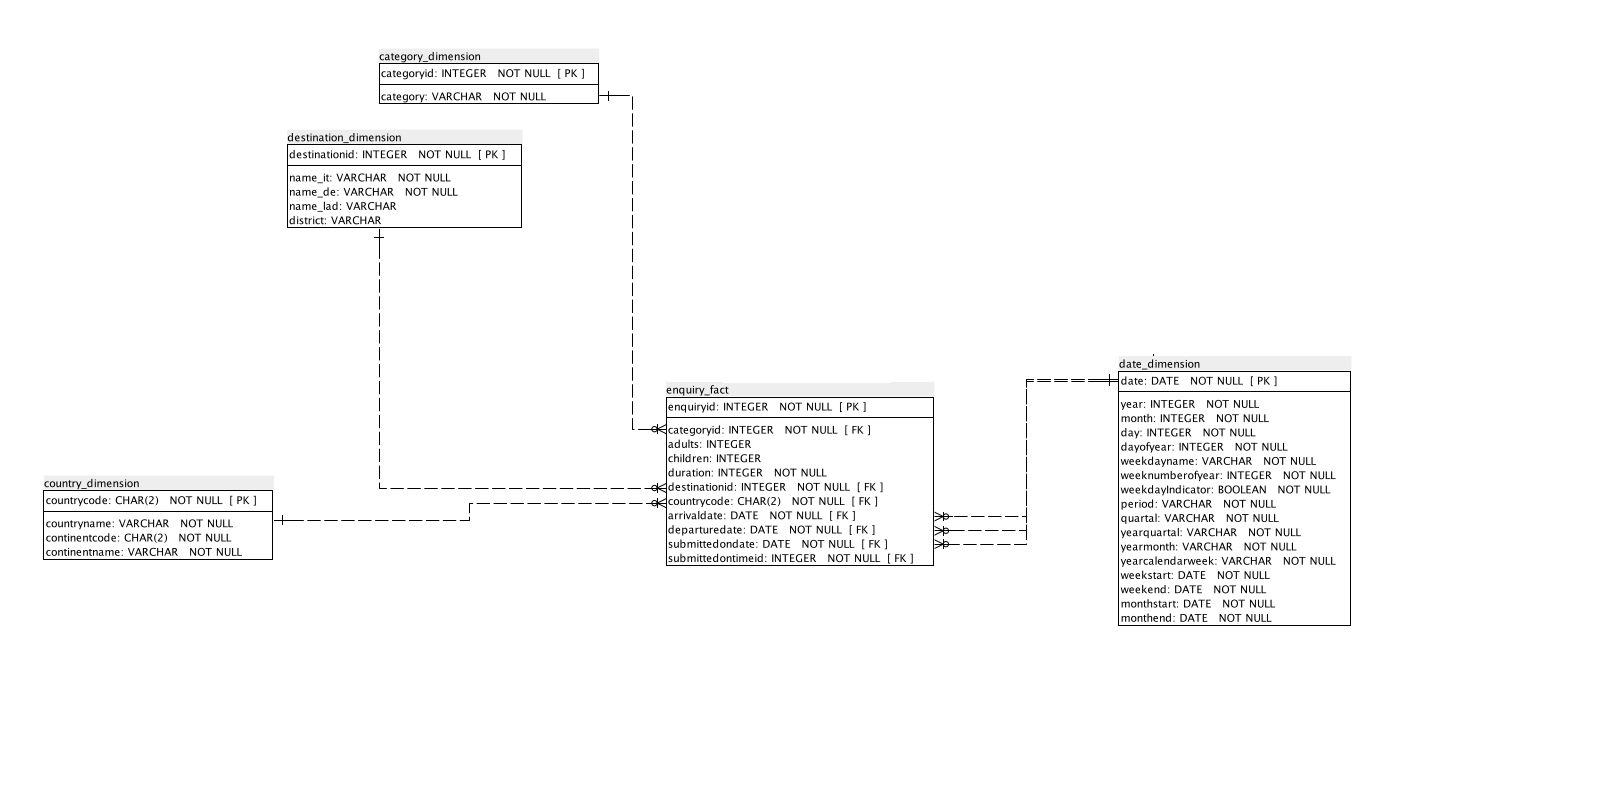
\includegraphics[scale=0.5,width=\textwidth]{img/schema_fact_inquiry.jpg}
	\caption{Relational schema of the fact INQUIRY (only dimensions and fact tables shown that have an \textsc{Ontop} mapping to the ontology)}
	\label{fig:schema_fact_inquiry}
\end{figure}

\begin{figure}
	\centering
	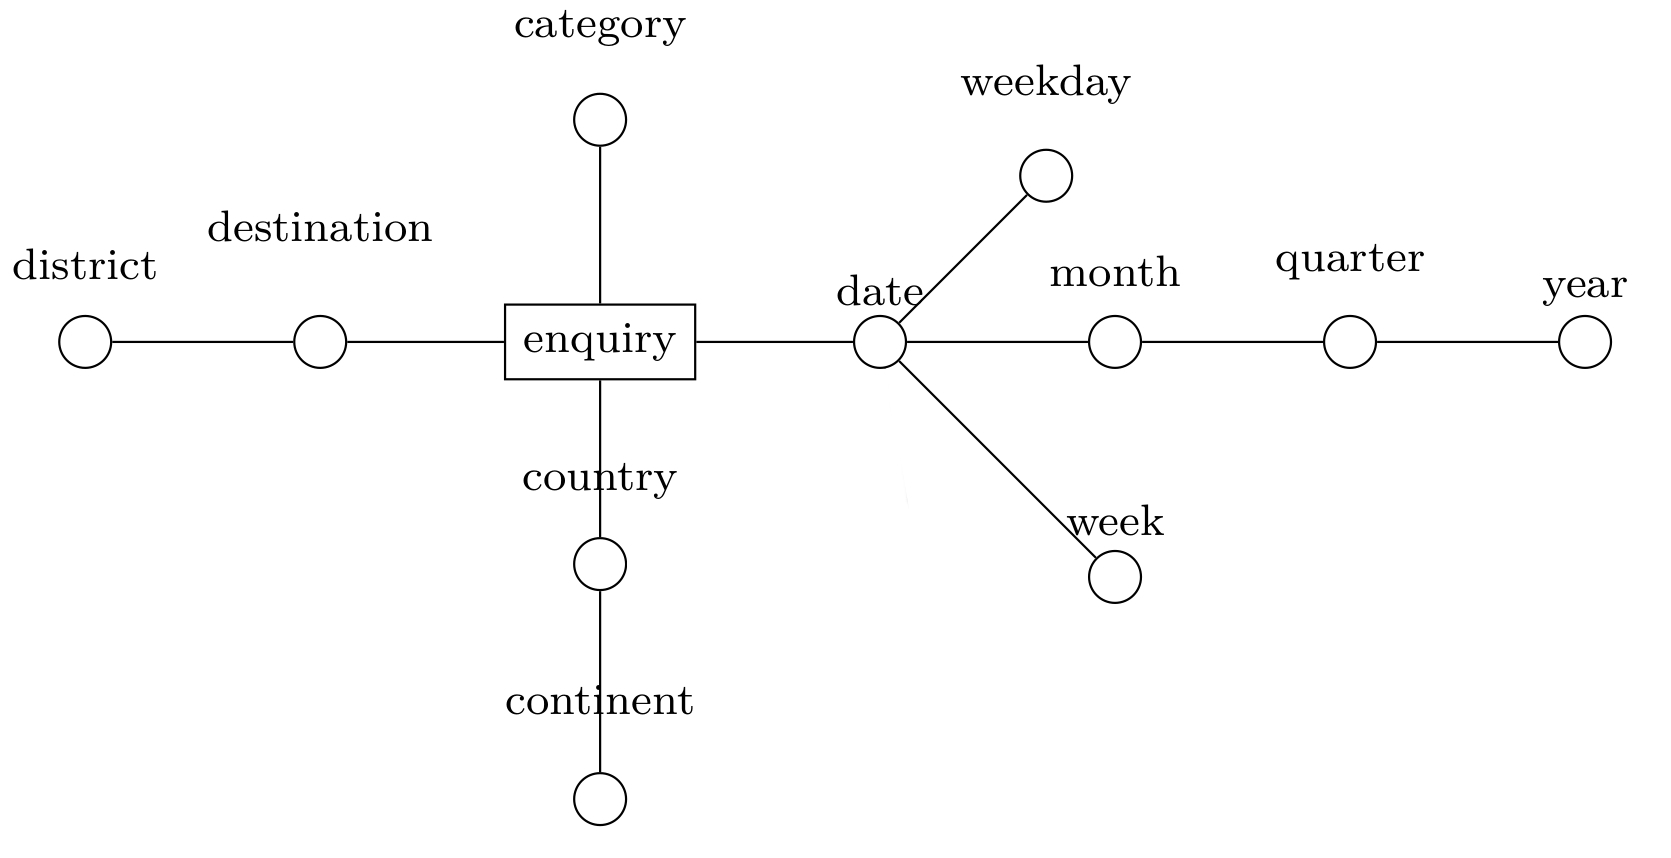
\includegraphics[scale=0.35,width=\textwidth]{img/fact_schema.jpg}
	\caption{Fact schema of the fact INQUIRY (only dimensions and fact tables shown that have an \textsc{Ontop} mapping to the ontology)}
	\label{fig:fact_schema}
\end{figure}

	% !TeX spellcheck = en_US

\section{Architecture of the System}
\label{chapter:architecture}

This system's architecture is made of four components: First, a PostgreSQL database to store the fact table and dimension tables. The schema of these tables have already been explained in Chap.~\ref{chapter:schema}. Second, an \textsc{Ontop} platform to query this relational database as a virtual RDF graph. Hereby, I generated an OWL file, to describe the ontology graph with its data properties, object properties, and classes. At the same time, I generated an OBDA file to define the data connection parameters to PostgreSQL, and to describe the mappings from a given SPARQL query to its SQL counterpart. Both files have been build with the \textsc{Prot\'eg\'e} ontology graph editor. Third, the \textsc{rdf4j} library (formerly known as Sesame) to connect to and query RDF data. The connection has been made to \textit{\url{http://dbpedia.org}}. 

The reason to have this simple architecture is that I tried several other things before, to find out, that not all things are currently possible that I wanted to use for this project. However, it was interesting to try and see all the possibilities and restrictions that exists currently. 

\subsection{Trials and errors}
With this chapter I want to address the report requirement: \textit{Lessons learned from the project / advantages and drawbacks of the
semantic technologies}.

During the development I tried to integrate both data sources, namely the local tourism ontology, and the remote dbpedia SPARQL endpoint, into a single federation setup. I installed \textsc{Jetty} and the \textsc{OpenRDF workbench} for it. Then, I configured the mentioned sources as two SPARQL endpoints. In addition, I wanted to generated a \textit{Federation Store}. However, it did not work, since I got two errors. First, an \textit{Virtuoso Error: No permission} to select a certain table. Unfortunately, I can not reproduce this error while writing the report. Hence, I cannot provide more details. Second, the following Java exception:
\begin{lstlisting}[language=]
org.openrdf.repository.RepositoryException: org.openrdf.repository.RepositoryException: Unable to get namespaces from Sail
	at org.openrdf.http.client.HTTPClient.handleHTTPError(HTTPClient.java:953)
	at org.openrdf.http.client.HTTPClient.sendTupleQueryViaHttp(HTTPClient.java:718)
	at org.openrdf.http.client.HTTPClient.getTupleQueryResult(HTTPClient.java:643)
	at org.openrdf.http.client.SesameHTTPClient.getNamespaces(SesameHTTPClient.java:321)
	at org.openrdf.http.client.SesameHTTPClient.getNamespaces(SesameHTTPClient.java:302)
	...
\end{lstlisting}

Afterwards, I thought of keeping both endpoints separate, and use the \texttt{SERVICE} keyword to integrate both sources into a single query, but again, I got a \textit{not supported} error message.
\begin{lstlisting}[language=]
Query evaluation error: it.unibz.inf.ontop.model.OBDAException: Error rewriting and unfolding into SQL 
\end{lstlisting}

The third idea I had, was to reproduce data warehouse operations, such as drill down and drill up. Unfortunately, I got the error from \textsc{Ontop}, that aggregation and grouping is currently not supported. Therefore, I thought of retrieving all data and grouping it in Java. However, the data is huge, and therefore these operations take some time calculating. I found out, that these clauses are part of SPARQL v1.1. In contrast, \textsc{Ontop} supports SPARQL v1.0 only. The aggregation algorithm I wrote in Java is a simple sort-hash-algorithm. That is, I restrict the data input such that every attribute must be sorted. Then, I scan through the input data and build groups from the first attribute to the last. As long as a group stays the same I increment a counter, if the group changes the output tuple is made by writing all group members and the counter, and the counter is afterwards set to zero. All the hash techniques are handled by \texttt{java.util.HashMap}. Finally, if the input is not sorted an error exception is thrown, and all calculations stopped.

	% !TeX spellcheck = en_US

\section{Semantic Techniques}
\label{chapter:semantictechniques}

Figure~\ref{fig:ontology} depicts the hierarchical structure of my tourist inquiries ontology. It contains three main concepts, namely \textit{Category}, \textit{Location}, and \textit{Tourist Action}. As you can see I have neglected time and date dimensions present in the data warehouse model. I decided to develop this application in an iterative manner, starting from a simple model with a few concepts only, but with a complex hierarchical structure connecting them. Unfortunately, I did not had the time to integrate time/date later. Each concept pointed by an arrow is a super-class of the concept connected to it. 

\subsection{Classes}

The all-to-all connection pattern seen under Category is due to the fact, that the data source generated only 5 categories, where the \textit{Hotel} category is an umbrella term for \textit{Pension}, \textit{Garni}, \textit{Pub}, and \textit{Residence}. However, I thought of dividing these concepts, because the domain experts could separate them later on more easily. These concepts are defined as \textsc{Equivalent To} each other, and as \textsc{subclass of} Category. However, such details are not shown in the \textsc{OwlViz} graph.

The \textit{Location} hierarchy shows first the general concept of locations in the world, and then different granularities, such as \textit{Continent}, \textit{Country}, \textit{Province}, \textit{Touristic District}, and \textit{City or town}, where the latest one is defined as possible destination for tourists. In addition, I have defined a \textit{Ladin Town} as a \textit{City or town} with a ladin name.

The \textit{Tourist action} class contains currently only \textit{Inquiry} as subclass, which contains five defined classes \textit{Farm Inquiry}, \textit{Other Accommodation Inquiry}, \textit{Private Inquiry}, and a disjoint union of \textit{Inquiries for Hotel with 1-3 stars} and \textit{Inquiries for Hotels with 4-5 stars} composing a superclass \textit{Hotel Inquiries}.

\begin{figure}[h]
\centering
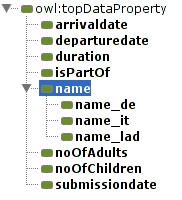
\includegraphics[width=0.3\linewidth]{img/data_property_hierarchy}
\caption{Data property hierarchy}
\label{fig:data_property_hierarchy}
\end{figure}

\begin{figure}[h]
\centering
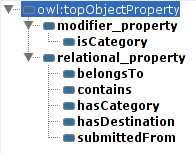
\includegraphics[width=0.3\linewidth]{img/object_property_hierarchy}
\caption{Object property hierarchy}
\label{fig:object_property_hierarchy}
\end{figure}

The inquiry class (referring to the inquiry fact table of the data warehouse) contains several data properties, such as \textit{name}, \textit{number of adults}, \textit{number of children}, \textit{date of submitting the inquiry}, \textit{arrival date}, \textit{departure date}, and \textit{duration of the holiday}. The whole hierarchy can be seen in Fig.~\ref{fig:class_inquiry_properties}. Each property is used exactly once for each inquiry, although some are defined as optional in the data warehouse design document. However, we can set it to a exact cardinality of one, because the value are always non-null (for instance, set to zero if numeric, and not defined). Finally, the \textit{name} properties are \textit{functional}.

\begin{figure}[h]
\centering
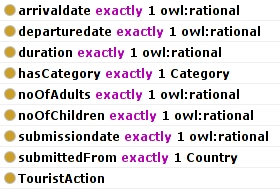
\includegraphics[width=0.4\linewidth]{img/class_inquiry_properties}
\caption{Inquiry data properties and constraints (modeled as \textsc{subclass~of} constraint)}
\label{fig:class_inquiry_properties}
\end{figure}

Subclasses of \textit{Inquiry} are defined as \textsc{Equivalent To} a class expression. For example, the \textit{Farm Inquiry} is equivalent to the following definition:
\begin{lstlisting}
Enquiry and (isCategory only Farm)
\end{lstlisting}
All other subclasses are defined analogous, except for \textit{Hotel Inquiry} which is a disjoint union of \textit{Hotel123Inquiry} and \textit{Hotel45Inquiry}, which are defined as follows
\begin{lstlisting}
HotelEnquiry and (isCategory only Hotel123)
HotelEnquiry and (isCategory only Hotel45)
\end{lstlisting}

\begin{sidewaysfigure}
	\centering
	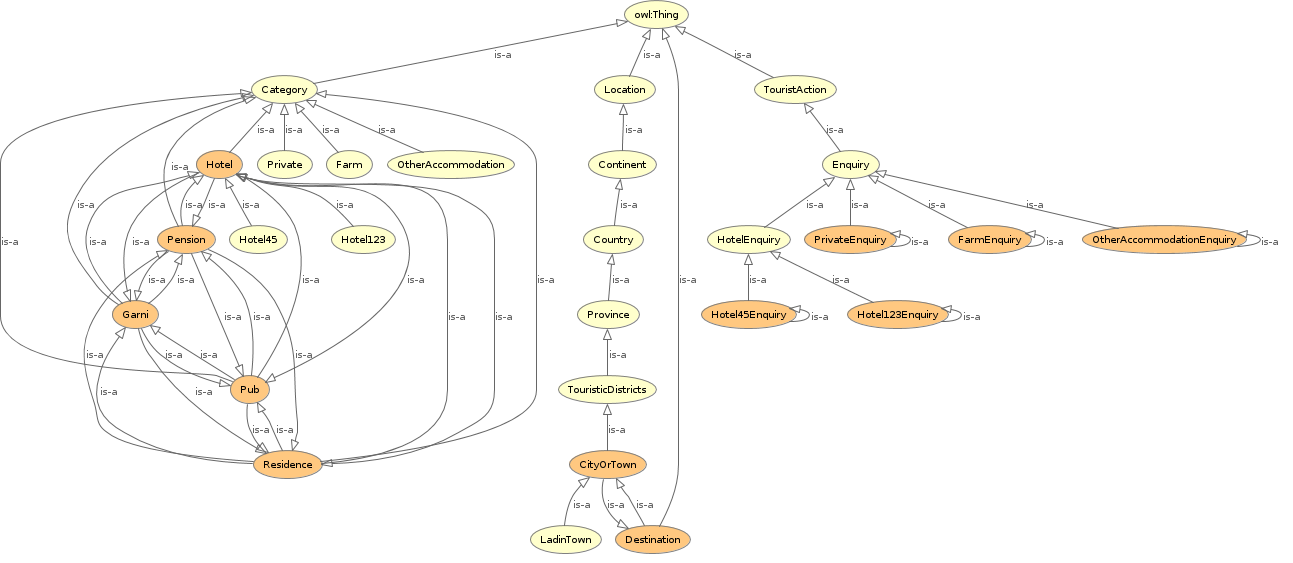
\includegraphics[width=\textwidth]{img/ontology.png}
	\caption{\textsc{OwlVIZ} representation of my tourist inquiries ontology}
	\label{fig:ontology}
\end{sidewaysfigure}





	% !TeX spellcheck = en_US

\section{Implementation}
\label{chapter:implementation}

\textit{NB: The code can be found on the UNIBZ gitlab server\footnote{ \url{https://gitlab.inf.unibz.it/peter-moser/semanticTechnology-tourism}}.}

Figure~\ref{fig:GUI} shows the graphical user interface of my Java application. It shows a list of executable queries on the left below the menu bar. The play-button (top-left) executes queries loaded and shown in the middle textual view. This queries can be temporarily modified, that is, no load and save functionality has been implemented yet. After execution the translated SQL query is shown on the right-hand-side (see text field with gray background). The label below the query code view shows some information (or errors) thrown out by the backend. Last, the bottom contains a table which presents the query results. If a cell of this table is double-clicked, a dialog pops up. This dialog shows some information (if available) about the clicked literal. Currently, only destination literals have a corresponding \textit{dbpedia.org} mapping.

\begin{figure}
\centering
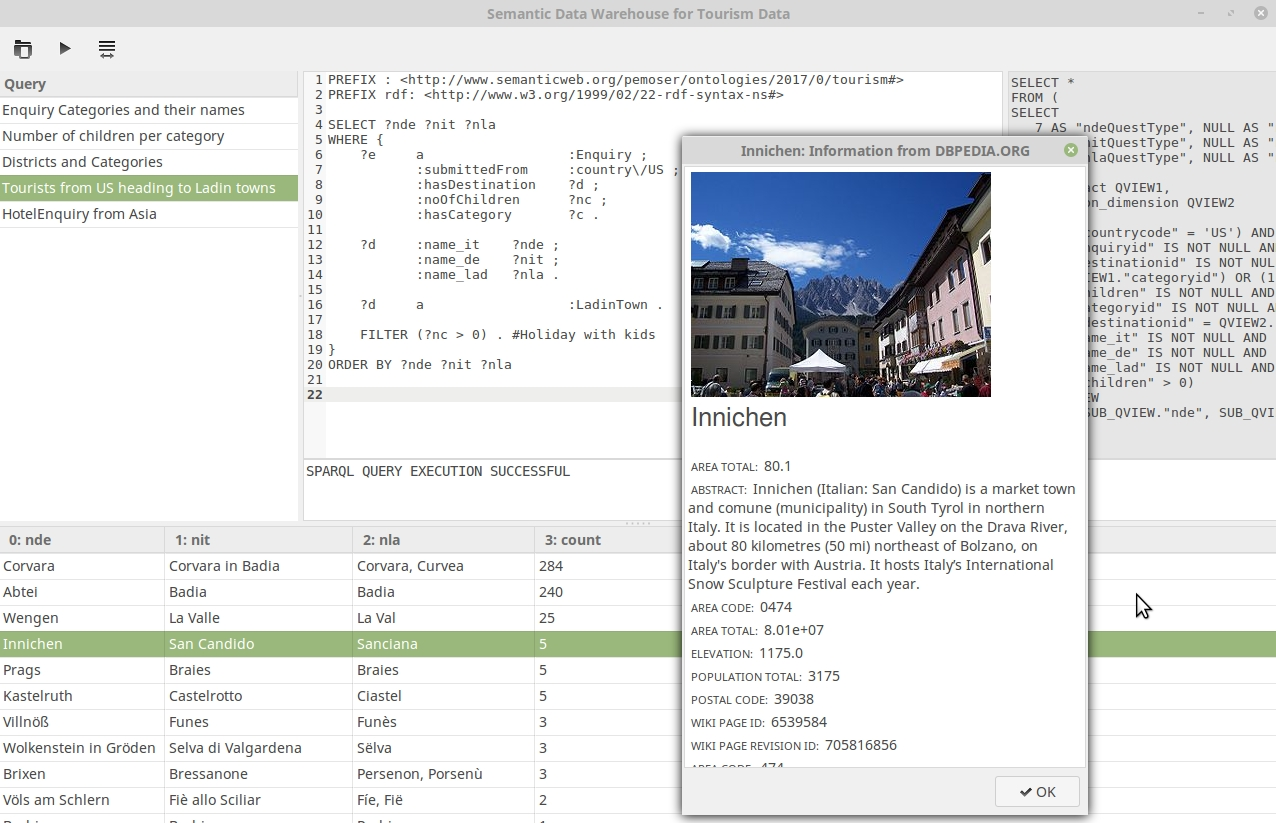
\includegraphics[width=0.7\linewidth]{img/GUI}
\caption{Graphical User Interface of my Semantic Java Application}
\label{fig:GUI}
\end{figure}

\subsection{Used libraries and tools}

In summary I used the following:
\begin{itemize}
\item GTK+ bindings for Java, namely \textit{java-gnome}
\item \textsc{Ontop} framework
\item \textsc{RDF4J} library
\item \textsc{PostgreSQL} as database
\item \textsc{Protege} workbench to generate the OWL and OBDA files
\end{itemize}

I generated the user interface with GTK+ bindings for Java, namely \textsc{java-gnome}, and the GUI builder \textsc{Glade}. Then I searched for the SPARQL query file parser used in the \textsc{Ontop} plugin for \textsc{Protege}, but did not find it immediately. Therefore, I thought to quickly write a preliminary version my self. It parses a \textit{tourism.q} or \textit{dbpedia.q} file, and gives for each \textit{QueryItem} the code section.  Secondly, I reused the \textit{org.semanticweb.ontop.examples.QuestOWLExample} class as a basis to build my own query executor. Third, I wrote an GTK-event-handler to connect to a remote SPARQL repository, and retrieve all literals from a single query. If the \textit{long IRI} toggle is deactivated, I fetch the prefixes from the SPARQL query, and replace each IRI inside the result with its prefix. The following chapter describes how I used \textsc{Quest} and \textsc{RDF4J}.

On the development side, I used \textsc{Eclipse}, \textsc{Maven}, and \textsc{Git}.

\subsection{Applying Semantic Techniques}
In this section I will explain which semantic techniques I used within this project, and how it got implemented in Java. I start with \textsc{Ontop}, \textsc{Quest}, and the \textsc{Owl Api}.

I loaded the \textit{.owl} file and \textit{.obda} file, and created an \textit{OWLOntology}, and a \textit{OBDAModel} from them. Then I had to prepare the configuration for Quest. I reused the code an created a ''Virtual ABox'' mode setup. This means,  that \textsc{Ontop} gets as input a set of mappings (given by the OBDA file), and does just translate the given SPARQL queries over the ontology from the OWL file to SQL queries over the database (in our case PostgreSQL). In contrast, a ''Classic ABox'' mode would need an ontology and data triples to ABOX assertions\footnote{\url{https://github.com/ontop/ontop/wiki/Ontop-Preferences}}. However, the former method is used here.

Then, I generate a quest OWL factory with the previously defined preferences, and obda model, to get a reasoner over this ontology, which can be used to create an statement for \textsc{Quest} out of a given SPARQL query string.

Finally, I retrieved the translated SQL query with \textit{getUnfolding}, and executed the statement with the \textit{executeTuple} method. The result set contained then a signature, that is, all targets from the defined select list of the query (projection), and the bindings to each OWL object, that is, the values of the result.

In addition, I used the \textsc{Rdf4J} framework as follows:
\begin{itemize}
\item Opened connection to \textit{\url{http://dbpedia.org/sparql}} endpoint
\item Executed the query in two steps: First, by preparing a executable statement with \textit{prepareTupleQuery}, and second, by executing it with \textit{evaluate}
\item The result set provides an iterator interface, where I could retrieve all binding sets step-by-step
\item I fetched the thumbnail of each town given by the \textit{thumbnail} value of each retrieved tuple (the redirection of that URL gave some troubles initially, but I could solve that issue by reading the HTTP headers, and issuing a second fetch request.)
\end{itemize}

\subsection{Problem with Semantic Techniques}
I had two problems with the structure of the ontology graph of \textit{dbpedia.org}. On one hand, some information is redundant and therefore multiple instances of the same key/value pair showed up in the results. I have seen that this happened because the IRI was different, but contained the same key finally. For instance, \textit{populationTotal} has two IRIs, namely
\begin{lstlisting}
http://dbpedia.org/property/populationTotal
http://dbpedia.org/ontology/populationTotal
\end{lstlisting}

On the other hand, no unique literal pattern has been defined for city/town names. For example, the town with a German name \textit{Kastelruth} has an Italian correspondence of \textit{Castelrotto,\_South\_Tyrol}. In addition, some predicates are defined for English \textit{dbpedia.org} entries, that do not exist in other \textit{dpbedia.org} versions for other languages. The unique identifier, that I is common in Italy to identify cities or towns is the so-called ISTAT code, from the national statistics Bureau, but there is no such entry in dbpedia. However, I have found a SPARQL endpoint for ISTAT at last, which may be a better endpoint for my needs. Hopefully, I can continue with my project later on to make it really useful.
	% !TeX spellcheck = en_US

\section{Conclusion and Future work}
\label{chapter:conclusion}

This project could be extended in several ways. First, it would be nice to incorporate a non-semantic drill down and drill up view upon the data warehouse with standard OLAP SQL queries.

Then, for each dimension, it would be nice to have a functionality to define mappings to external SPARQL endpoints, depending on an ontology class hierarchy defined with ONTOP and PROTEGE. For example, defining an ontology for the destination dimension to find new attributes for them. A SPARQL connection to the ISTAT, DBPEDIA, and other endpoints could be defined to explore the connected ontologies first. Then, after deciding upon an attribute (for instance, elevation of a town), an additional mapping could define how to extend the relational database. The semantic techniques would hereby help to find new ideas, and available data and semantic connections between concepts in the real-world.

Last, a completeness measure would be needed to see how many tuples of a dimension could be filled with a predefined mapping. For instance, if some towns do not have an \textit{elevation} defined, or if the mappings are not uniquely defined and some towns have more than one \textit{elevation} to be assigned. 

In general, during my development I had some ideas about how semantic technologies could help data warehouse designers to make the best out of their business. However, it is not easy to combine different ontologies (and SPARQL endpoints) in technical and semantical (i.e., missing in-common IRIs) sense. Nevertheless, I liked this project a lot, because it gave me new insights in how-to explore an area with querying tools, and how close philosophical and technical worlds can come.

%	\newpage
%	\appendix
%	\section{Appendix: Listings}
%	\label{app:listings}	
%	\lstinputlisting[
%		caption={SPARQL queries generated with Protege.},
%		label={lst:sparql}, 
%		language=SPARQL]
%		{../ontology/tourism_v2.q}

\end{document}
